\documentclass[a4paper,10pt]{report}
\usepackage[english]{babel}
\usepackage[utf8]{inputenc}
\usepackage{listings}
\usepackage{enumitem}
\usepackage{graphicx}

\graphicspath{{./figures}}


\title{A-FMM User Guide}
\author{Marco Passoni}
\date{}

\begin{document}

\maketitle

\chapter{Reference Guide}
In this chapter a detailed explanation of the module is provided. For each sub-module a summary of the classes and function involved can be found, together with details on the most common functions.
\section{Module composition}
The A-FMM module in turn composed by different submodules:
\begin{itemize}
\item creator module: Contain the creator class, used to define the dielectric costant of the single layer.   
\item layer module: Contain the layer class, used to solve the Maxwell equation inside each single layer. It requires a creator instance to be initialized.
\item scattering module: Contain the S\_matrix class. All method for scattering matrix creation and manipulation are here implemented.  
\item satck module: Contain the stack class, used to calculate the Scattering Matrix and related quantities of the hole structure. It is initialize from a collection of layer instances.
\item sub\_sm module: Contains auxiliary function that are called in more than one module. It is non loaded by default when loading A\_FMM.
\end{itemize}

\section{Scattering module}
\subsection{S\_matrix class}
\subsubsection{Definition ad initialization}
This class contains the definition of the scattering matrix object and all method for scattering matrix manipulation. The scattering matrix is an object relating the amplitudes of the incoming end outgoing modes of a structure. It presets itself as following:
\begin{equation} \label{eq:S_matrix_def}
\left[
\begin{array}{c}
u' \\
d  \\
\end{array} 
 \right] = \left[
 \begin{array}{cc}
S_{11} & S_{12} \\
S_{21} & S_{22} \\
\end{array}
 \right]
 \left[
\begin{array}{c}
u \\
d' \\
\end{array} 
\right]
\end{equation}
following the convention of figure \ref{fig:SM_conv}.
\begin{figure}
\centering
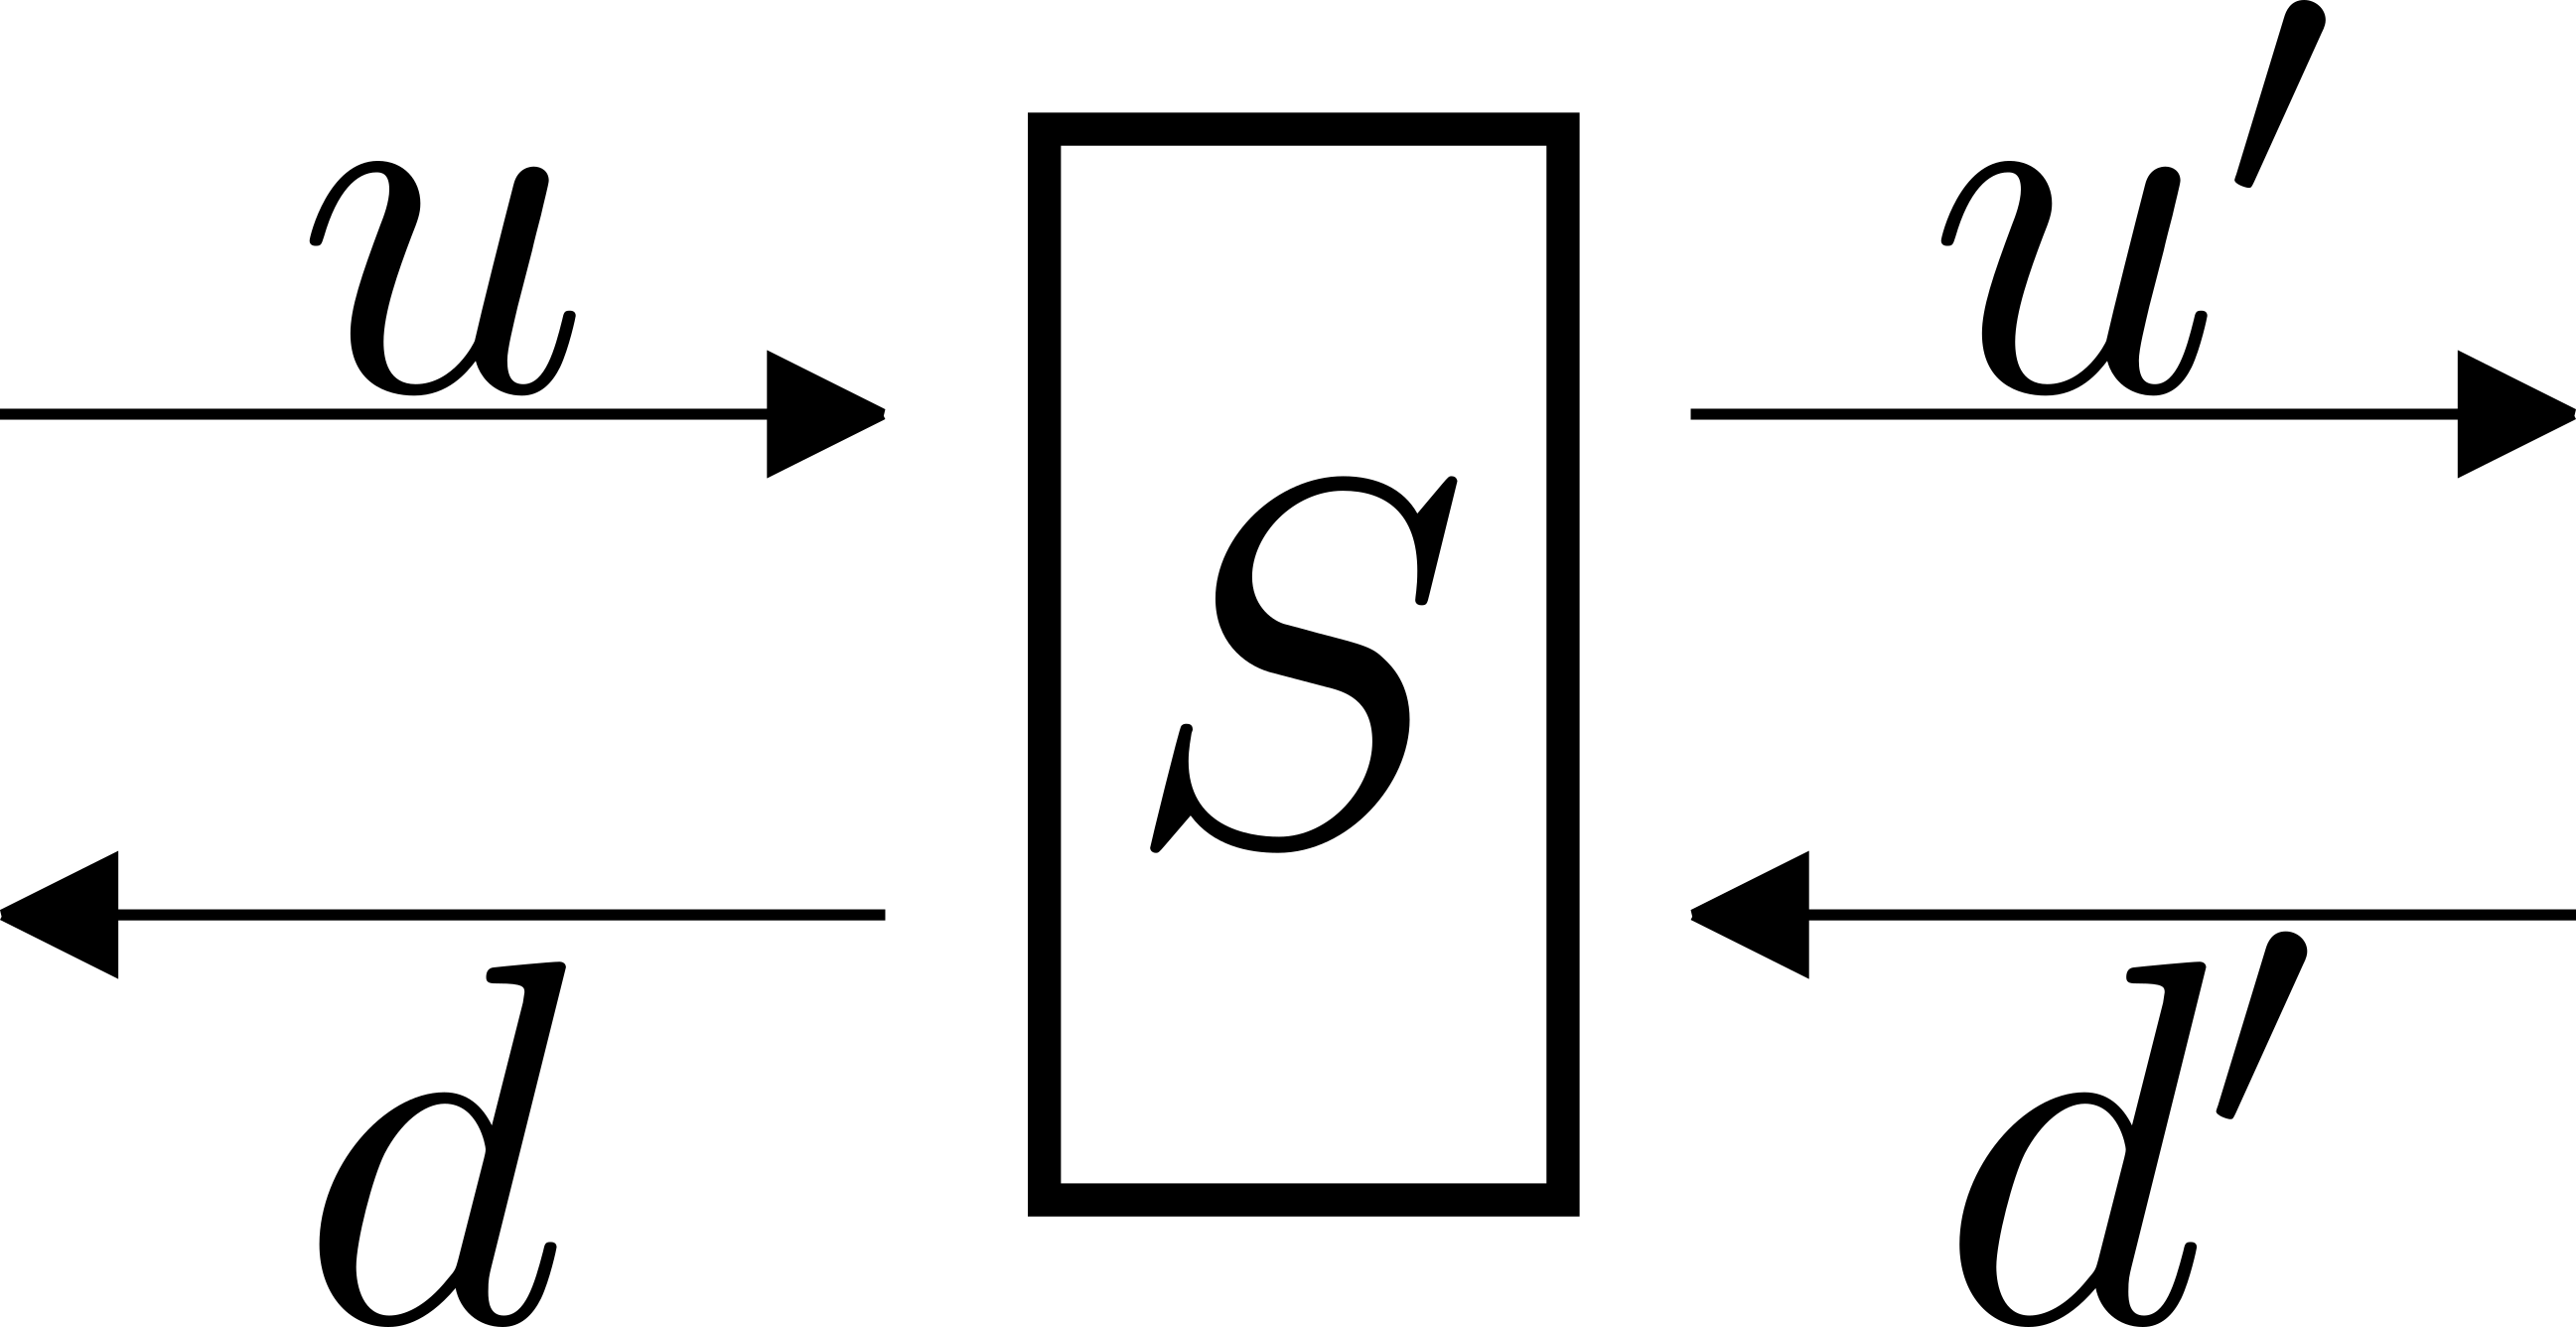
\includegraphics[width=0.5\textwidth]{figures/S.png}
\caption{Convention adopted for the scattering matrix formalism.} \label{fig:SM_conv}
\end{figure}
An instance is initialized as:
\begin{lstlisting}[language=Python]
S=S_matrix(N)
\end{lstlisting}
where \texttt{N} is the dimension of the four $N \times N$ matrices composing the scattering matrix. Each of this matrix is saved as an \texttt{numpy.ndarray} as an attribute of the S\_matrix object. For example to the $(1,2)$ element of the $S_{21}$ matrix is accessed as \texttt{S.S21[1,2]}.

\subsubsection{Method}
\begin{lstlisting}[language=Python,basicstyle=\ttfamily\Large]
add(s)
\end{lstlisting}
Takes as input an other instance of the S\_matrix class s, which is then joined to the right to the scattering matrix that calls the method.

\begin{lstlisting}[language=Python,basicstyle=\ttfamily\Large]
add_left(s)
\end{lstlisting}
Same as \texttt{add} but s matrix is joined to the left.

\begin{lstlisting}[language=Python,basicstyle=\ttfamily\Large]
add_uniform(lay,d)
\end{lstlisting}
Takes as input:
\begin{itemize}[noitemsep,topsep=0pt,parsep=0pt,partopsep=0pt]
\item \texttt{lay}: An instance of the layer class;
\item \texttt{d}: A float representing the thickness of the layer.
\end{itemize}
This method creates the scattering matrix for propagation trough a layer \texttt{lay} of thickness \texttt{d}, and then joins it to the right of the scattering matrix that calls the method.

\begin{lstlisting}[language=Python,basicstyle=\ttfamily\Large]
add_uniform_left(lay,d)
\end{lstlisting}
Same as \texttt{add\_uniform} but joins to the left.





\section{Layer Module}
\subsection{Layer class}
\subsubsection{Initialization}
This module contain the layer class, which is responsable for definition of the single layer inside the scattering matrix approach. It also contains the methods for adding the coordinate transform an plotting of the mode fields. It is initialized as: 
\begin{lstlisting}[language=Python]
lay=layer(Nx,Ny,creator,Nyx=1.0)
\end{lstlisting}
with the following parameters:
\begin{itemize}[noitemsep,topsep=0pt,parsep=0pt,partopsep=0pt]
\item \texttt{Nx,Ny}: Trucation order respectively in $x$ and $y$ direction. Actual number of plane waves is $(2N_x+1)(2N_y+1)$.
\item \texttt{creator}: The creator instance describing the dielectric function.
\item \texttt{Nyx}: Ratio between the cell period in $y$ and $x$ direction (default is 1.0).
\end{itemize}
When initializing the layer class all the matrices involve in the eigenvalue problem for the layer are created.
\subsubsection{Methods}
\begin{lstlisting}[language=Python,basicstyle=\ttfamily\Large]
trasform(ex=0,ey=0)
\end{lstlisting}
Add the real coordinate transform.
\begin{itemize}[noitemsep,topsep=0pt,parsep=0pt,partopsep=0pt]
\item \texttt{ex,ey}: Respectively the width of the untransformed region in $x$ and $y$ direction. If not specified transformation in not applied in that direction.
\end{itemize}

\begin{lstlisting}[language=Python,basicstyle=\ttfamily\Large]
trasform_complex(ex=0,ey=0)
\end{lstlisting}
Add the complex coordinate transform simulating PML boundary conditions. 
\begin{itemize}[noitemsep,topsep=0pt,parsep=0pt,partopsep=0pt]
\item \texttt{ex,ey}: Respectively the width of the untransformed region in $x$ and $y$ direction. If not specified transformation in not applied in that direction.
\end{itemize}

\begin{lstlisting}[language=Python,basicstyle=\ttfamily\Large]
mode(k0,kx=0.0,ky=0.0,v=1)
\end{lstlisting}
Solve the eigenvalue problem of the layer.
\begin{itemize}[noitemsep,topsep=0pt,parsep=0pt,partopsep=0pt]
\item \texttt{k0}: Energy of the mode
\item \texttt{kx,ky}: Respectively the lateral wavevector in the $x$ and $y$ direction (in unit of inverse of the period).
\item  \texttt{v}: If equal to 0 only eigenvalue are calculated. Useful when interested only in propagation constant of the mode of the single layer. Default is 1.
\end{itemize}
create three new attributes of the class layer:
\begin{itemize}[noitemsep,topsep=0pt,parsep=0pt,partopsep=0pt]
\item \texttt{W}: Vector of the eigenvalues (effective indexes of modes squared). 
\item \texttt{V}: Matrix of electric eigenvectors of the modes. \texttt{V[:,i]} is the vector to the $i^{th}$ mode.
\item \texttt{VH}: Matrix of magnetic eigenvectors of the modes. Same convention as \texttt{V}.
\end{itemize}

\begin{lstlisting}[language=Python,basicstyle=\ttfamily\Large]
eps_plot(pdf=None,N=200,s=1.0)
\end{lstlisting}
Plot dielectric function profile reconstructed from fourier transform.
\begin{itemize}[noitemsep,topsep=0pt,parsep=0pt,partopsep=0pt]
\item \texttt{pdf}: Name of the pdf file used to save the figure (string, without the .pdf).
\item \texttt{N}: Width in pixel of the cell. Default 200.
\item \texttt{s}: Number of fundamental cells plotted. Default 1.
\end{itemize}

\begin{lstlisting}[language=Python,basicstyle=\ttfamily\Large]
plot_E(pdf,i,N=100,s=1,func=np.abs)
\end{lstlisting}
Plot electric field profile of selected mode.
\begin{itemize}[noitemsep,topsep=0pt,parsep=0pt,partopsep=0pt]
\item \texttt{pdf} Instances of the PdfPages class. Specify pdf file where to save field.
\item \texttt{i} Number of mode to plot. Mode are ordered in decreasing effective index. Numeration start at 1.
\item \texttt{N} Width in pixel of the cell. Default 100.
\item \texttt{s} Number of fundamental cells plotted. Default 1.
\item \texttt{func} Since field is complex, function to apply to field before plotting. Default is abs. Useful can be real, imag, angle. 
\end{itemize}

\begin{lstlisting}[language=Python,basicstyle=\ttfamily\Large]
plot_H(pdf,i,N=100,s=1,func=np.abs)
\end{lstlisting}
Plot magnetic field profile of selected mode. Same inputs as \texttt{plot\_E}.

\begin{lstlisting}[language=Python,basicstyle=\ttfamily\Large]
plot_field(pdf,i,N=100,s=1,func=np.abs)
\end{lstlisting}
Plot both electric and magnetic field profile of selected mode. Same inputs as \texttt{plot\_E}. 

\begin{lstlisting}[language=Python,basicstyle=\ttfamily\Large]
get_field(x,y,i,func=np.abs)
\end{lstlisting}
Return field of selected mode at selected point. 
\begin{itemize}[noitemsep,topsep=0pt,parsep=0pt,partopsep=0pt]
\item \texttt{x,y} Coordinate of the point in which to calculate fields.
\item \texttt{i} Number of mode to plot. Mode are ordered in decreasing effective index. Numeration start at 1.
\item \texttt{func} Since field is complex, function to apply to field before plotting. Default is abs. Useful can be real, imag, angle. 
\end{itemize}
Return 1-dim array of length 4 containing in order: Ex,Ey,Hx,Hy

\begin{lstlisting}[language=Python,basicstyle=\ttfamily\Large]
get_P_norm()
\end{lstlisting}
Calculate z component of Poynting vector, used in the scattering matrix algorithm to normalize correctly reflection ad transmission.
The values of Poynting vector are then stored in the new attribute \texttt{P\_norm}.

\begin{lstlisting}[language=Python,basicstyle=\ttfamily\Large]
T_interface(lay)
\end{lstlisting}
Takes in input a different instance of the layer class. Return the transfer matrix representing the interface between the layer that calls the method and the layer given ad input.  The obtained matrix is an instance of \texttt{numpy.ndarray}. 

\begin{lstlisting}[language=Python,basicstyle=\ttfamily\Large]
T_prop(d)
\end{lstlisting}
Takes in input a float value \texttt{d} representing the thickness of the layer. Return the transfer matrix of the propagation trough a thickness d of the layer that calls the method. Could generate numerical instabilities.  The obtained matrix is an instance of \texttt{numpy.ndarray}. 

\begin{lstlisting}[language=Python,basicstyle=\ttfamily\Large]
interface(lay)
\end{lstlisting}
Takes in input a different instance of the layer class. Return the scattering matrix representing the interface between the layer that calls the method and the layer given ad input.  The obtained matrix is an instance of \texttt{S\_matrix}. 




\end{document}
\begin{lstlisting}[language=Python,basicstyle=\ttfamily\Large]
\end{lstlisting}
\begin{itemize}[noitemsep,topsep=0pt,parsep=0pt,partopsep=0pt]
\item \texttt{Nx,Ny}
\end{itemize}
